\documentclass{beamer}\usepackage{graphicx, color}
%% maxwidth is the original width if it is less than linewidth
%% otherwise use linewidth (to make sure the graphics do not exceed the margin)
\makeatletter
\def\maxwidth{ %
  \ifdim\Gin@nat@width>\linewidth
    \linewidth
  \else
    \Gin@nat@width
  \fi
}
\makeatother

\IfFileExists{upquote.sty}{\usepackage{upquote}}{}
\definecolor{fgcolor}{rgb}{0.2, 0.2, 0.2}
\newcommand{\hlnumber}[1]{\textcolor[rgb]{0,0,0}{#1}}%
\newcommand{\hlfunctioncall}[1]{\textcolor[rgb]{0.501960784313725,0,0.329411764705882}{\textbf{#1}}}%
\newcommand{\hlstring}[1]{\textcolor[rgb]{0.6,0.6,1}{#1}}%
\newcommand{\hlkeyword}[1]{\textcolor[rgb]{0,0,0}{\textbf{#1}}}%
\newcommand{\hlargument}[1]{\textcolor[rgb]{0.690196078431373,0.250980392156863,0.0196078431372549}{#1}}%
\newcommand{\hlcomment}[1]{\textcolor[rgb]{0.180392156862745,0.6,0.341176470588235}{#1}}%
\newcommand{\hlroxygencomment}[1]{\textcolor[rgb]{0.43921568627451,0.47843137254902,0.701960784313725}{#1}}%
\newcommand{\hlformalargs}[1]{\textcolor[rgb]{0.690196078431373,0.250980392156863,0.0196078431372549}{#1}}%
\newcommand{\hleqformalargs}[1]{\textcolor[rgb]{0.690196078431373,0.250980392156863,0.0196078431372549}{#1}}%
\newcommand{\hlassignement}[1]{\textcolor[rgb]{0,0,0}{\textbf{#1}}}%
\newcommand{\hlpackage}[1]{\textcolor[rgb]{0.588235294117647,0.709803921568627,0.145098039215686}{#1}}%
\newcommand{\hlslot}[1]{\textit{#1}}%
\newcommand{\hlsymbol}[1]{\textcolor[rgb]{0,0,0}{#1}}%
\newcommand{\hlprompt}[1]{\textcolor[rgb]{0.2,0.2,0.2}{#1}}%

\usepackage{framed}
\makeatletter
\newenvironment{kframe}{%
 \def\at@end@of@kframe{}%
 \ifinner\ifhmode%
  \def\at@end@of@kframe{\end{minipage}}%
  \begin{minipage}{\columnwidth}%
 \fi\fi%
 \def\FrameCommand##1{\hskip\@totalleftmargin \hskip-\fboxsep
 \colorbox{shadecolor}{##1}\hskip-\fboxsep
     % There is no \\@totalrightmargin, so:
     \hskip-\linewidth \hskip-\@totalleftmargin \hskip\columnwidth}%
 \MakeFramed {\advance\hsize-\width
   \@totalleftmargin\z@ \linewidth\hsize
   \@setminipage}}%
 {\par\unskip\endMakeFramed%
 \at@end@of@kframe}
\makeatother

\definecolor{shadecolor}{rgb}{.97, .97, .97}
\definecolor{messagecolor}{rgb}{0, 0, 0}
\definecolor{warningcolor}{rgb}{1, 0, 1}
\definecolor{errorcolor}{rgb}{1, 0, 0}
\newenvironment{knitrout}{}{} % an empty environment to be redefined in TeX

\usepackage{alltt}
\usetheme{Stats}
\setbeamercovered{transparent}
\usepackage{color}
\usepackage{hyperref}
  \hypersetup{
  	colorlinks=true
		linkcolor=black
		}
\usepackage{url}
\usepackage{graphics}
\usepackage{tikz}
\usepackage{booktabs}

\usepackage[buttonsize=1em]{animate}





%%%%%%%%%%%%%%%%%%%%%%%%%%%%%%%% Title Slide %%%%%%%%%%%%%%%%%%%%%%%%%%
\title[]{Intro to Social Science Data Analysis \\[1cm] Lecture 7: Overview of Statistical Inference}
\author[]{
    \href{mailto:gandrud@yonsei.ac.kr}{Christopher Gandrud}
}
\date{\today}


\begin{document}

\frame{\titlepage}

\section[Outline]{}
\frame{\tableofcontents}

%%%%%%%%%%% Assignment 2 Reminder
\section{Assignment 2}
\frame{
  \frametitle{Assignment 2}
  \textbf{Due:} Friday 19 October \\[0.25cm]
  
  \textbf{Describe} at least \textbf{3} variables in a data set.\\[0.25cm]
  {\small{
    You need to select a \textbf{range of descriptive statistical tools}. The tools should include both \textbf{numerical descriptive statistics} and \textbf{graphics}.\\[0.25cm]

    These tools should describe the variables':
    \begin{itemize}
      \item<1-> central tendency,
      \item<1-> variation,
      \item<1-> their relationships with the other variables.
    \end{itemize}

    The descriptions need to be discussed \textbf{in paragraph form}. \\[0.25cm]

    The description must be \textbf{reproducible}. So you should email me the link to a Dropbox folder with:
    \begin{itemize}
      \item<1-> the \texttt{.csv} data set,
      \item<1-> the \texttt{.Rmd} R markdown file,
      \item<1-> the final \texttt{.html} file.
    \end{itemize}
  }}
}

%%%%%%%%%%%%%%% Recap
\section{Recap}
\frame{
	\frametitle{Principles of Quantitative Graphics (1)}
{\Large{What are some of the goals that quantitative graphics should try to achieve?}}
}

\frame{
  \frametitle{Principles of Quantitative Graphics (2)}
  {\Large{What are some things you should not do in quantitative graphics? \\[0.5cm]
  In particular, how does the {\bf{data-ink ratio}} help us create effective graphics? \\[0.5cm]
  Remember:}}
  \[
    \mathrm{Data\:Ink\:Ratio = \frac{data-ink}{total\:ink}}
  \]
}

\frame{
  \frametitle{What is wrong with this graph?}
  \begin{center}
    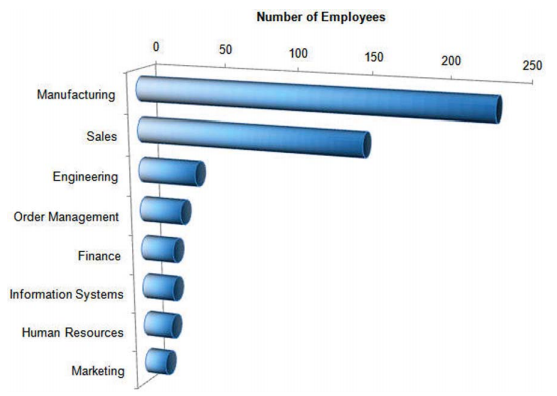
\includegraphics[scale=0.4]{figure/Employees3D.png} \\
    {\tiny{Source: \url{http://www.perceptualedge.com/articles/visual_business_intelligence/rules_for_using_color.pdf}}}
  \end{center}
}

\frame{
  \frametitle{Improved}
  \begin{center}
    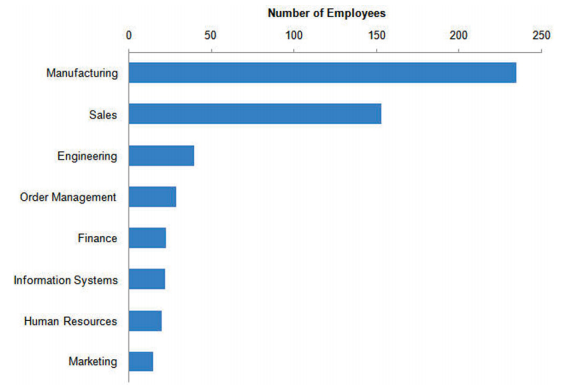
\includegraphics[scale=0.4]{figure/EmployeesFlat.png} \\
    {\tiny{Source: \url{http://www.perceptualedge.com/articles/visual_business_intelligence/rules_for_using_color.pdf}}}
  \end{center}
}

\section{Take a Sample}
\begin{frame}[fragile]
  \frametitle{Today's Data Download}
\begin{knitrout}
\definecolor{shadecolor}{rgb}{0.969, 0.969, 0.969}\color{fgcolor}\begin{kframe}
\begin{alltt}
\hlcomment{# Load package RCurl}
\hlfunctioncall{library}(RCurl)

\hlcomment{# Create URL object for OpenIntro data}
url <- \hlfunctioncall{paste}(\hlstring{"https://raw.github.com/christopher"},
             \hlstring{"gandrud/Introduction_to_Statistics_"},
             \hlstring{"and_Data_Analysis"},
             \hlstring{"_Yonsei/master/Lectures/Lecture7/"},
             \hlstring{"OpenIntroData/run10.txt"}, sep = \hlstring{""})

\hlcomment{# Download data}
Run10 <- \hlfunctioncall{getURL}(url, ssl.verifypeer = FALSE)

\hlcomment{# Convert Run10 to data.frame}
Run10 <- \hlfunctioncall{read.table}(\hlfunctioncall{textConnection}(Run10),
                    sep = \hlstring{"\textbackslash{}t"}, header = TRUE)
\end{alltt}
\end{kframe}
\end{knitrout}

\end{frame}

\begin{frame}[fragile]
  \frametitle{Today's Variables}
\begin{knitrout}
\definecolor{shadecolor}{rgb}{0.969, 0.969, 0.969}\color{fgcolor}\begin{kframe}
\begin{alltt}
\hlfunctioncall{names}(Run10)
\end{alltt}
\begin{verbatim}
## [1] "place"    "time"     "pace"     "age"     
## [5] "gender"   "location" "state"    "divPlace"
## [9] "divTot"
\end{verbatim}
\end{kframe}
\end{knitrout}


  {\bf{Today}} we will use these variables (from Diaz et al. (2011, Ch. 4)):
  \begin{table}
    \begin{tabular}{l p{4cm}}
      \hline
      Variable & Description \\[0.3cm] 
      \hline\hline
      \texttt{time} & ten mile run time, minutes \\
      \texttt{age} & age of runner in years \\
      \hline
    \end{tabular}
  \end{table}
\end{frame}

\begin{frame}[fragile]
  \frametitle{Random Sample}
{\large{Our data contains the {\bf{entire population}} of 16,974 runners who finished the 2009 Cherry Blossom 10 Mile Run in Washington, DC. \\[0.5cm]
  But imagine, however, that we only have a {\bf{simple random sample}} of 100 runners.}}
\end{frame}

\begin{frame}[fragile]
  \frametitle{Illustrate Random Sample}
\begin{knitrout}
\definecolor{shadecolor}{rgb}{0.969, 0.969, 0.969}\color{fgcolor}

{\centering \animategraphics[,controls,loop]{1}{figure/SamplingAnimation}{1}{50}

}


\end{knitrout}

\end{frame}

\begin{frame}[fragile]
  \frametitle{Take random sample}
\begin{knitrout}
\definecolor{shadecolor}{rgb}{0.969, 0.969, 0.969}\color{fgcolor}\begin{kframe}
\begin{alltt}
\hlcomment{# Find number of runners in population}
\hlfunctioncall{nrow}(Run10)
\end{alltt}
\begin{verbatim}
## [1] 16924
\end{verbatim}
\begin{alltt}

\hlcomment{# Take a random sample of 100 runners}
Run10Samp <- Run10[\hlfunctioncall{sample}(1:\hlfunctioncall{nrow}(Run10), 100,
                          replace=FALSE),]

\hlcomment{# Find number of runners in sample}
\hlfunctioncall{nrow}(Run10Samp)
\end{alltt}
\begin{verbatim}
## [1] 100
\end{verbatim}
\end{kframe}
\end{knitrout}

\end{frame}

\begin{frame}[fragile]
  \frametitle{Sample Distribution of \texttt{time}}
\begin{knitrout}
\definecolor{shadecolor}{rgb}{0.969, 0.969, 0.969}\color{fgcolor}\begin{kframe}
\begin{alltt}
\hlfunctioncall{hist}(Run10Samp$time)
\end{alltt}
\end{kframe}

{\centering 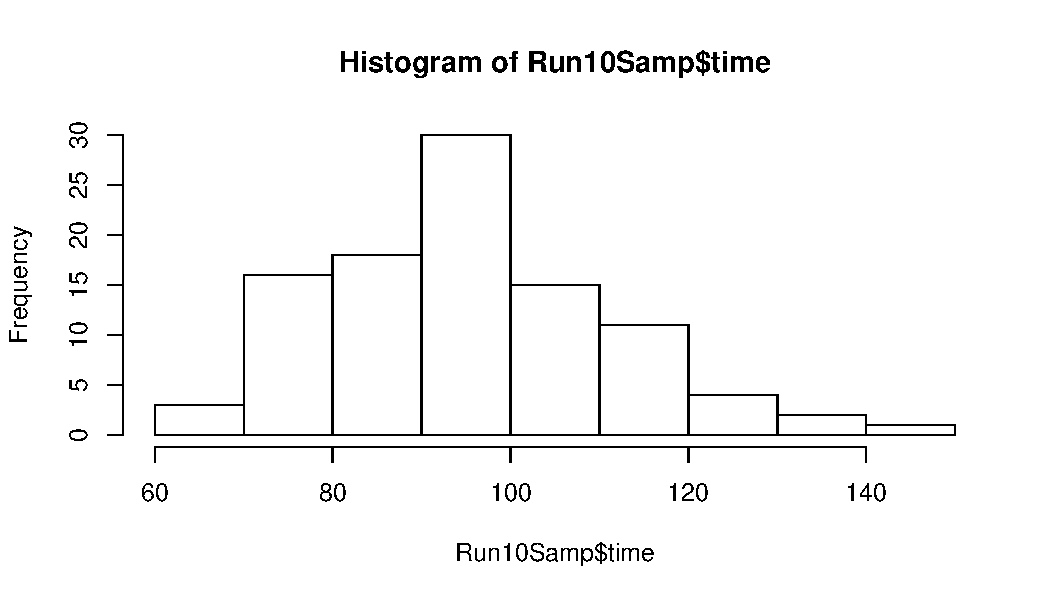
\includegraphics[width=\maxwidth]{figure/HistSampTime} 

}


\end{knitrout}

\end{frame}

\begin{frame}[fragile]
  \frametitle{Sample Distribution of \texttt{age}}
\begin{knitrout}
\definecolor{shadecolor}{rgb}{0.969, 0.969, 0.969}\color{fgcolor}\begin{kframe}
\begin{alltt}
\hlfunctioncall{hist}(Run10Samp$age)
\end{alltt}
\end{kframe}

{\centering 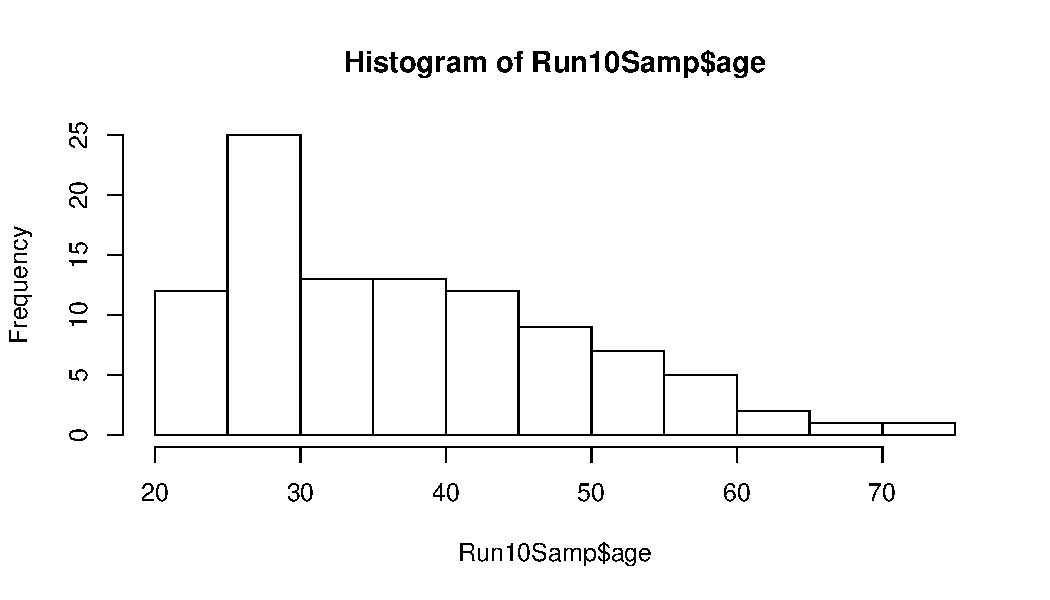
\includegraphics[width=\maxwidth]{figure/HistSampAge} 

}


\end{knitrout}

\end{frame}

%%%%%%%%%%%%% Point Estimates \& Population Parameters
\section{Point Estimates \& Population Parameters}
\frame{
  \frametitle{The Question}
  \begin{center}
    {\Large{How similar is the sample to the population?\\[1cm]
    In other words, how {\bf{representative}} is the sample? \\[1cm]
    In other other words, what can we {\bf{infer}} about the population from the sample?}}
  \end{center}
}

\frame{
  \frametitle{More specifically: Means}
  {\Large{Today we are particularly interested in how similar the {\bf{sample means}} $\bar{x}$ are to the {\bf{true population means $\mu$ for:}} \\[0.25cm]
  \begin{itemize}
    \item<2-> average \texttt{time} it took to complete the race,
    \item<3-> average \texttt{age} of the runners.}}
  \end{itemize}
}

\frame{
  \frametitle{Inference}
  {\Large{To answer these questions we will need tools of {\bf{statistical inference}}. \\[1cm]
  Today we will learn the basics of statistical inference. \\[0.5cm]
  We will use these tools throughout the rest of the course and statistics. \\[0.5cm]
  Statistical inference is key for linking our (sampled) data to what we care about: questions about populations.}}
}

\begin{frame}[fragile]
  \frametitle{The Sample Means}
    {\Large{Lets find our sample means.\\[0.5cm]
    Time:}}
\begin{knitrout}
\definecolor{shadecolor}{rgb}{0.969, 0.969, 0.969}\color{fgcolor}\begin{kframe}
\begin{alltt}
\hlfunctioncall{mean}(Run10Samp$time)
\end{alltt}
\begin{verbatim}
## [1] 97.01
\end{verbatim}
\end{kframe}
\end{knitrout}


  {\Large{Age:}}
\begin{knitrout}
\definecolor{shadecolor}{rgb}{0.969, 0.969, 0.969}\color{fgcolor}\begin{kframe}
\begin{alltt}
\hlfunctioncall{mean}(Run10Samp$age)
\end{alltt}
\begin{verbatim}
## [1] 35.53
\end{verbatim}
\end{kframe}
\end{knitrout}

\end{frame}

\frame{
  \frametitle{Point Estimates (1)}
  \begin{center}
{\Large{These are {\bf{point estimates}} of a {\bf{population parameter}}, the population mean.}}
  \end{center}
}

\begin{frame}[fragile]
  \frametitle{Point Estimates (2)}
  {\large{We can find point estimates of other parameters. \\[0.5cm]
  For example, lets find point estimates for the sample {\bf{standard deviation of the mean}} ($s$). (The population parameter of the standard deviation is usually written $\sigma$).\\[0.25cm]
  Time:}}
\begin{knitrout}
\definecolor{shadecolor}{rgb}{0.969, 0.969, 0.969}\color{fgcolor}\begin{kframe}
\begin{alltt}
\hlfunctioncall{sd}(Run10Samp$time)
\end{alltt}
\begin{verbatim}
## [1] 17.91
\end{verbatim}
\end{kframe}
\end{knitrout}


  {\large{Age:}}
\begin{knitrout}
\definecolor{shadecolor}{rgb}{0.969, 0.969, 0.969}\color{fgcolor}\begin{kframe}
\begin{alltt}
\hlfunctioncall{sd}(Run10Samp$age)
\end{alltt}
\begin{verbatim}
## [1] 10.67
\end{verbatim}
\end{kframe}
\end{knitrout}

\end{frame}

\frame{
  \frametitle{Summary of our Random Sample}
  \begin{table}
    \begin{tabular}{l  c c | c c}
    \hline
    Variable & $\bar{x}$ & $\mu$ & $s$ & $\sigma$ \\
    \hline\hline
    \texttt{time} & 97 & ? & 17.9 & ? \\
      \texttt{age} & 35.5 & ? & 10.7 & ? \\
      \hline
    
    \end{tabular}
  \end{table}
}

\frame{
  \frametitle{But\ldots}
  \begin{center}
  {\Large{But, {\bf{how do we know}} how {\bf{close}} the point estimates are to the real population parameters? \\[1cm] 
  Especially since taking {\bf{other samples}} we will create {\bf{different estimates}}.}}
  \end{center}
}

\begin{frame}[fragile]
  \frametitle{10000 Sample Means!}
{\Large{Lets find the sample mean of \texttt{time} ($\bar{x}_{time}$) in 10,000 samples!}}
\begin{knitrout}
\definecolor{shadecolor}{rgb}{0.969, 0.969, 0.969}\color{fgcolor}\begin{kframe}
\begin{alltt}
\hlcomment{# Find the sample means from 10,000 samples}
TimeSampMeans <- \hlfunctioncall{rep}(0, 10000)
  \hlfunctioncall{for} (i in 1:10000) \{
    Samp <- \hlfunctioncall{sample}(Run10$time, 100)
    TimeSampMeans[i] <- \hlfunctioncall{mean}(Samp)
    \}

\hlcomment{# Create a data frame object}
TimeSampMeans <- \hlfunctioncall{data.frame}(TimeSampMeans)
\end{alltt}
\end{kframe}
\end{knitrout}

\end{frame}


\begin{frame}[fragile]
    \frametitle{Distribution of the 10,000 Sample Means!}
\begin{knitrout}
\definecolor{shadecolor}{rgb}{0.969, 0.969, 0.969}\color{fgcolor}

{\centering 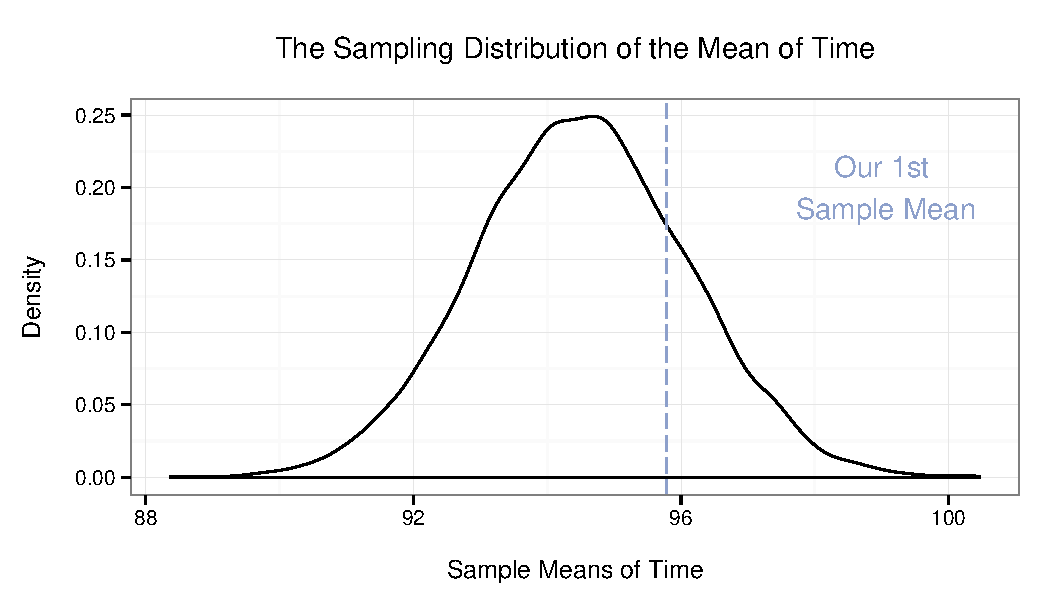
\includegraphics[width=\maxwidth]{figure/DistTimeSampleMean} 

}


\end{knitrout}

\end{frame}

\frame{
  \frametitle{Sampling distribution and the population mean}
  \begin{center}
    {\Large{The sampling distribution is {\bf{centered}} on the population mean!\\[1cm]
    Stated much more confusingly: the mean of the sampling distribution of the sample means is the population mean.}}
  \end{center}
}

\begin{frame}[fragile]
    \frametitle{Population Mean vs. Sample Means}
\begin{knitrout}
\definecolor{shadecolor}{rgb}{0.969, 0.969, 0.969}\color{fgcolor}

{\centering 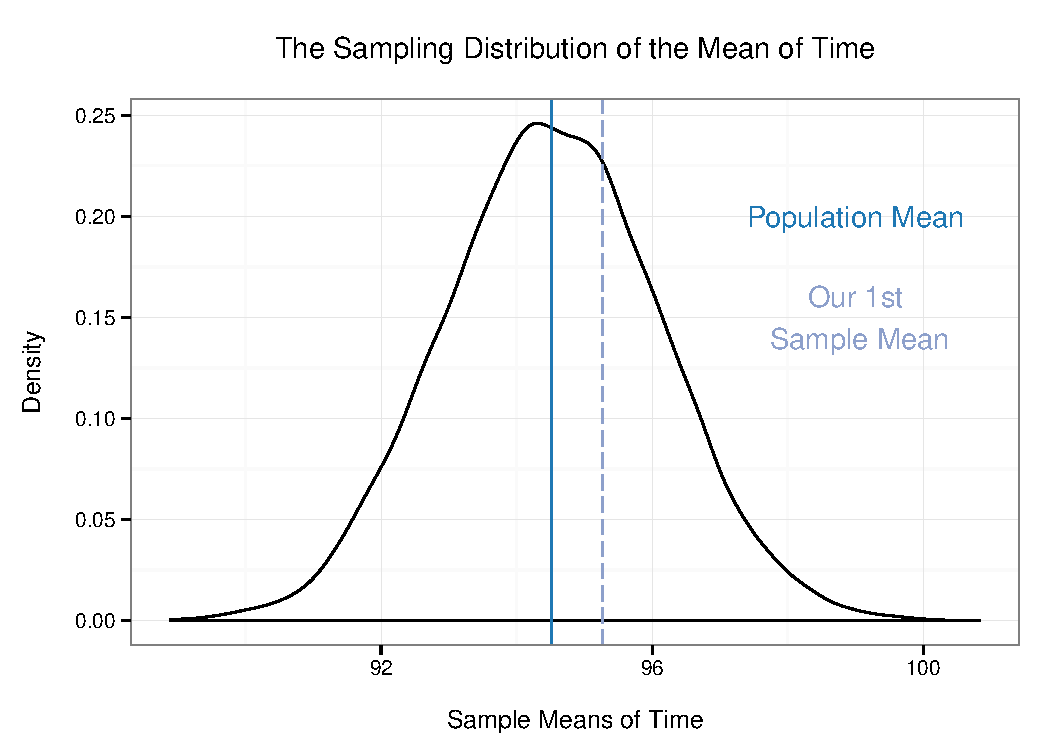
\includegraphics[width=\maxwidth]{figure/DistPopSampMean} 

}


\end{knitrout}

\end{frame}

\section{Standard Error}
\frame{
  \frametitle{Not solved yet.}
  \begin{center}
    {\Large{Ok, that is nice in theory, but what if we don't know the sampling distribution? \\[1cm]
    In real life we can't take 10,000 samples!}}
  \end{center}
}

\frame{
  \frametitle{Question\ldots}
  \begin{center}
    {\Large{Question: What would the sampling distribution of the sample mean look like if the sample size was 5,000 rather than 100?}}
  \end{center}
}

\begin{frame}[fragile]
    \frametitle{Comparing Sampling Distributions of $\bar{x}_{time}$ 100 vs. 5,000}
\begin{knitrout}
\definecolor{shadecolor}{rgb}{0.969, 0.969, 0.969}\color{fgcolor}

{\centering 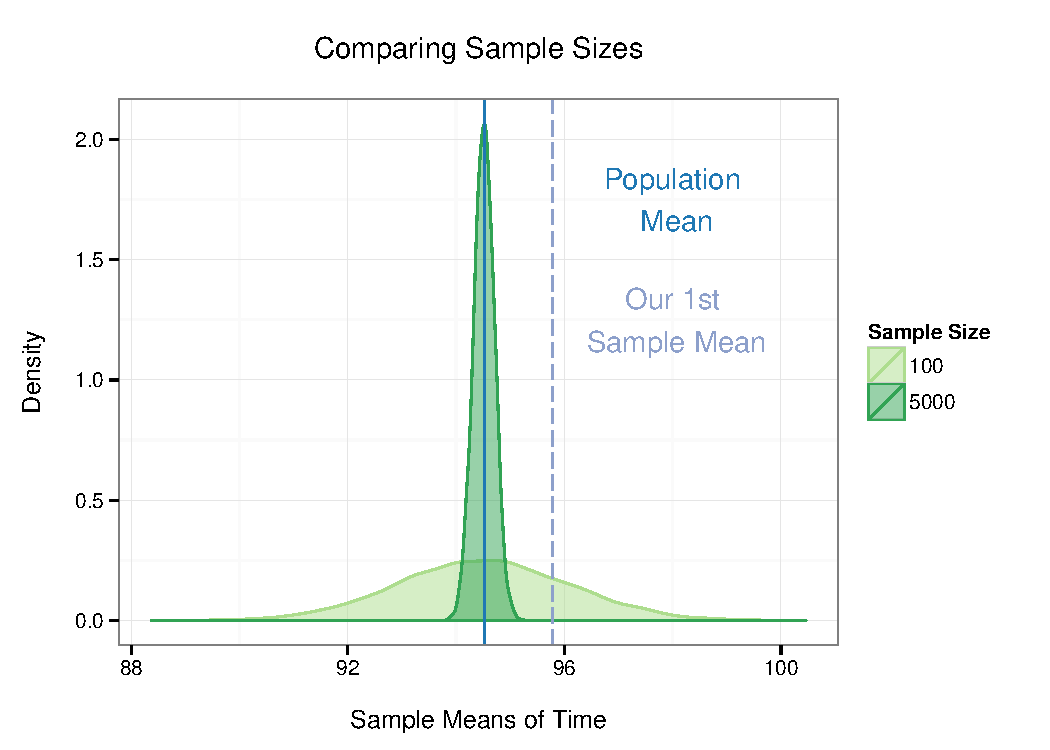
\includegraphics[width=\maxwidth]{figure/DistTimeSampleMean5000} 

}


\end{knitrout}

\end{frame}

\frame{
  \frametitle{Sample Size, Point Estimates, and Population Parameters}
  \begin{center}
    {\Large{The {\bf{likely distance}} between the sample mean and the population mean is related to the {\bf{sample size}} ($n$), \\[1cm]
    The {\bf{bigger}} the sample size, the more likely it is that the point estimate is {\bf{close}} to the population parameter.}}
  \end{center}
}

\frame{
  \frametitle{Variability}
  \begin{center}
    {\Large{Also, a {\bf{smaller sample standard deviation}} ($s$) indicates less variability $\rightarrow$ more likely that the point estimate is {\bf{close}} to the population parameter. \\[1cm]
    So\ldots}}
  \end{center}
}

\frame{
  \frametitle{Finally, the Standard Error!}
    {\Large{Standard Error ($SE$):}}
    \[
      SE = \frac{s}{\sqrt{n}}
    \] \\[1cm]
    Assuming that the observations are \emph{independent}, i.e. the value of one observation does not depend on the value of another observation.
}

\frame{
  \frametitle{SE and Uncertainty}
  {\Large{The {\bf{standard error}} is a {\bf{measure}} of our {\bf{uncertainty}} about how well the point estimate represents the population parameter.}}
}

\begin{frame}[fragile]
  \frametitle{The Standard Error of the Mean of \texttt{time}}
\begin{knitrout}
\definecolor{shadecolor}{rgb}{0.969, 0.969, 0.969}\color{fgcolor}\begin{kframe}
\begin{alltt}
\hlcomment{# Load plotrix}
\hlfunctioncall{library}(plotrix)

\hlcomment{# Calculate standard error of the mean of time}
\hlfunctioncall{std.error}(Run10Samp$time)
\end{alltt}
\begin{verbatim}
## [1] 1.791
\end{verbatim}
\end{kframe}
\end{knitrout}


  {\large{\texttt{Time} in our original sample with 100 observations had a sampling mean of 97 and a standard error of 1.8.
\end{frame}

%%%%%%%%%%%%% Confidence Intervals
\section{Confidence Intervals}
\frame{
  \frametitle{Um\ldots}
  {\Large{Um \ldots a sampling mean of 97 and a standard error of 1.8? \\[1cm]
  That's not very easy to understand.}}
}

\frame{
  \frametitle{We need something more useful.}
  {\Large{We need something that is more {\bf{intuitive}} to interpret. \\[0.5cm]
  Maybe a {\bf{range}} of likely population parameter values.}}
}

\frame{
  \frametitle{}
  \begin{center}
    {\LARGE{The Confidence Interval!}}
  \end{center}
}

\begin{frame}[fragile]
  \frametitle{Standard Error and the Sampling Distribution}
  {\Large{About {\bf{95\%}} of the time the population parameter will be within {\bf{about 2 standard errors}} of the point estimate. \\[1cm]
  95\% Confidence Interval ($CI$):}}
  \[
    CI = \mathrm{point\:estimate} \pm 2 * SE
  \]
\end{frame}




\frame{
  \frametitle{Central Limit Theorem}
  {\Large{Central Limit Theorem (informal definition):}} \\[0.5cm]
  If a sample has at least 50 independent observations, and the data is not extremely skewed, the distribution of the sampling mean closely approximates the normal distribution (Diaz et al., 2011, 151)) \\[0.5cm]
  So what? This lets our confidence interval be more {\bf{precise}}. 
  \[
    CI = \mathrm{point\:estimate} \pm 1.96 * SE
  \]
}

\begin{frame}[fragile]
  \frametitle{Confidence Interval Simulation}
\begin{knitrout}
\definecolor{shadecolor}{rgb}{0.969, 0.969, 0.969}\color{fgcolor}

{\centering \animategraphics[,controls,loop]{1}{figure/CIAnimation}{1}{50}

}


\end{knitrout}

\end{frame}

\begin{frame}[fragile]
  \frametitle{Visually Confirm Normally Distributed Time Data}
\begin{knitrout}
\definecolor{shadecolor}{rgb}{0.969, 0.969, 0.969}\color{fgcolor}\begin{kframe}
\begin{alltt}
\hlcomment{# Create Quantile-Quantile Plots}
\hlfunctioncall{qqnorm}(Run10Samp$time); \hlfunctioncall{qqline}(Run10Samp$time)
\end{alltt}
\end{kframe}

{\centering 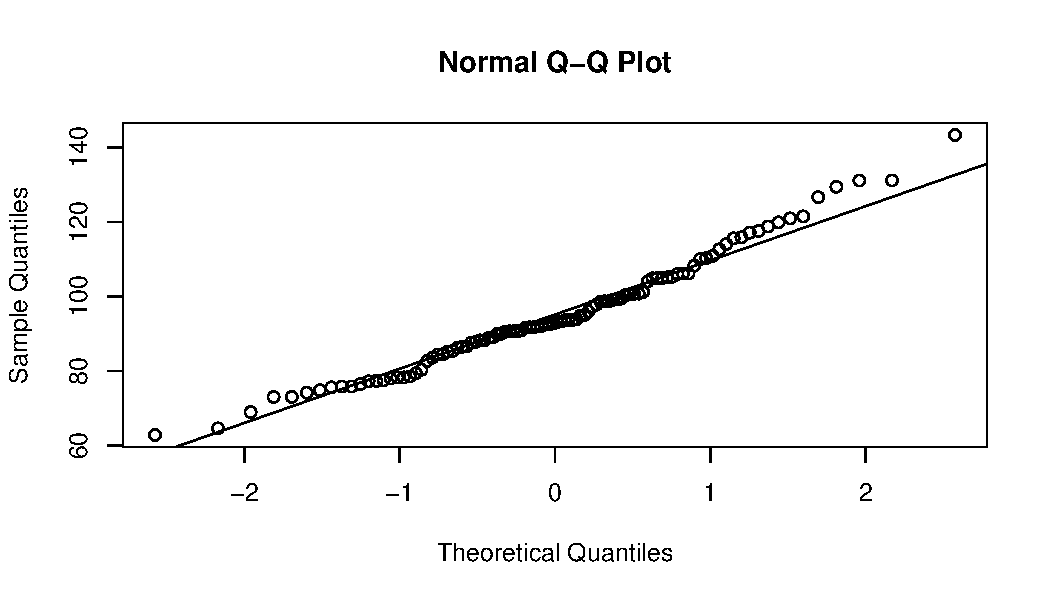
\includegraphics[width=\maxwidth]{figure/QQPlotTime} 

}


\end{knitrout}

\end{frame}

\begin{frame}[fragile]
  \frametitle{Visually Confirm Normally Distributed Age Data}
\begin{knitrout}
\definecolor{shadecolor}{rgb}{0.969, 0.969, 0.969}\color{fgcolor}\begin{kframe}
\begin{alltt}
\hlcomment{# Create Quantile-Quantile Plots}
\hlfunctioncall{qqnorm}(Run10Samp$age); \hlfunctioncall{qqline}(Run10Samp$age)
\end{alltt}
\end{kframe}

{\centering 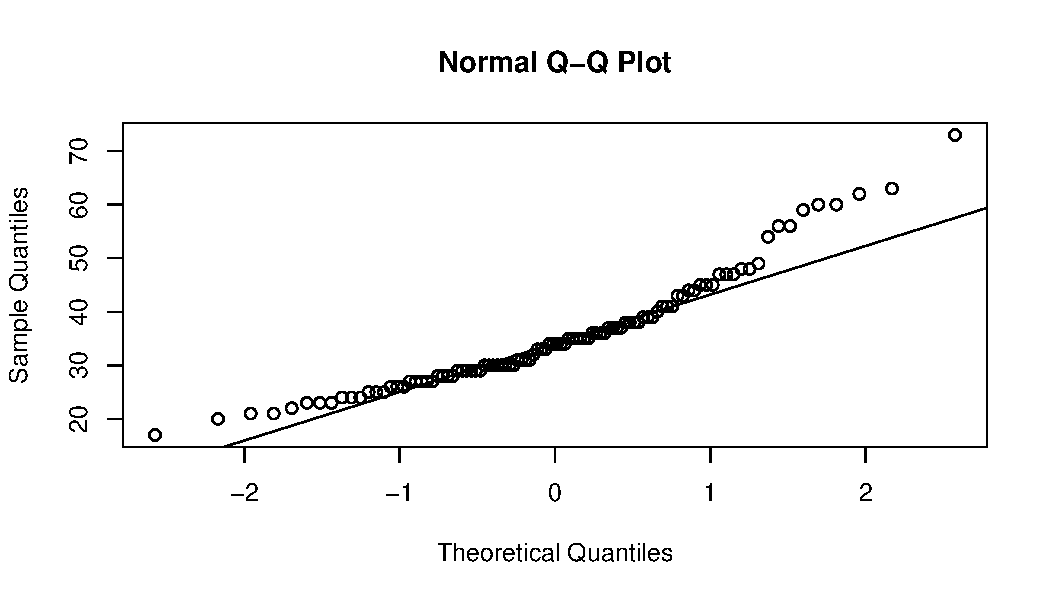
\includegraphics[width=\maxwidth]{figure/QQPlotAge} 

}


\end{knitrout}

\end{frame}

\frame{
  \frametitle{Independence}
{\Large{In general, observations from a simple random sample of {\bf{less than 10\% of the population}} will be independent.}}
}

\begin{frame}[fragile]
  \frametitle{Let's calculate some 95\% confidence intervals for \texttt{time}}
\begin{knitrout}
\definecolor{shadecolor}{rgb}{0.969, 0.969, 0.969}\color{fgcolor}\begin{kframe}
\begin{alltt}
\hlcomment{# Find Mean of time}
MeanTime <- \hlfunctioncall{mean}(Run10Samp$time)

\hlcomment{# Find Standard Error of the mean of time}
SETime <- \hlfunctioncall{std.error}(Run10Samp$time)

\hlcomment{# Lower CI}
LowerTime <- MeanTime - 1.96 * SETime

\hlcomment{# Upper CI}
UpperTime <- MeanTime + 1.96 * SETime
\end{alltt}
\end{kframe}
\end{knitrout}

\end{frame}

\begin{frame}[fragile]
\begin{knitrout}
\definecolor{shadecolor}{rgb}{0.969, 0.969, 0.969}\color{fgcolor}\begin{kframe}
\begin{alltt}
\hlcomment{# Show Confidence Intervals}
LowerTime
\end{alltt}
\begin{verbatim}
## [1] 93.5
\end{verbatim}
\begin{alltt}

UpperTime
\end{alltt}
\begin{verbatim}
## [1] 100.5
\end{verbatim}
\end{kframe}
\end{knitrout}




\end{frame}

\frame{
  \frametitle{Summary of our Parameter Estimates}
  \begin{table}
    \begin{tabular}{l  c c c | c}
    \hline
    Variable & Lower CI & Mean & Upper CI & Population Mean \\
    \hline\hline
    \texttt{time} & 93.5 & 97 & 100.5 & 94.5 \\
      \texttt{age} & 33.4 & 35.5 & 37.6 & 35.5 \\
      \hline
    
    \end{tabular}
  \end{table}
}

\begin{frame}[fragile]
  \frametitle{Alternative}



\begin{knitrout}
\definecolor{shadecolor}{rgb}{0.969, 0.969, 0.969}\color{fgcolor}

{\centering 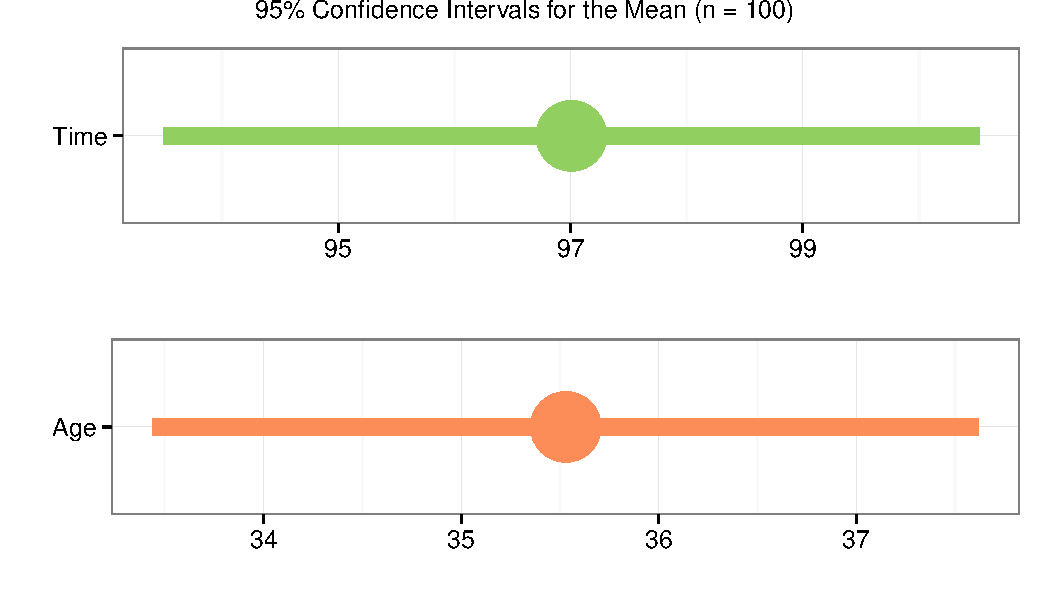
\includegraphics[width=\maxwidth]{figure/ConfIntPlot} 

}


\end{knitrout}

\end{frame}


\begin{frame}[allowframebreaks]
  \frametitle{References}
  Diaz, David M., Christopher D. Barr, and Mine \c{C}etinkaya-Rundel. 2011. OpenIntro Statistics. 1st ed. \url{http://www.openintro.org/stat/downloads.php}. \\[0.25cm] 
\end{frame}



\end{document}
